%
% 2_beispiel.tex -- Wellengleichung tatsächlich lösen mit der Methode
%
% (c) 2025 Roman Cvijanovic & Nicola Dall'Acqua, Hochschule Rapperswil
%
% !TEX root = ../../buch.tex
% !TEX encoding = UTF-8
%

\section{Rechenbeispiel\label{neuronal:section:rechenbeispiel}}
\kopfrechts{Rechenbeispiel}

In diesem Abschnitt wird die vorgestellte Methode auf die Wellengleichung in zwei Dimensionen und die Burgers-Gleichung in einer Dimension angewendet.
Der Ablauf ist analog zum Abschnitt \ref{neuronal:section:herleitung}:
\begin{enumerate}
    \item Definiere ein neuronales Netzwerk
    \item Generiere Datensätze für die Diskretierung
    \item Baue die Funktion $L(\vartheta)$ auf
    \item Minimiere $L(\vartheta)$
    \item Qualitätsbewertung mit $L(\vartheta)$ und $L^1(\vartheta)$
\end{enumerate}

\subsection{Wellengleichung}\label{neuronal:subsection:wellengleichung}
Die Gleichung ist
\begin{equation}
    \frac{\partial^2 u}{\partial t^2} = c^2 \left( \frac{\partial^2 u}{\partial x^2} + \frac{\partial^2 u}{\partial y^2} \right).
    \label{neuronal:wellengleichung}
\end{equation}
Die Konstante \( c \) ist die Verbreitungsgeschwindigkeit der Welle. Der Einfachheit halber wird $c = 1$ festgelegt.
Zusätzlich werden die folgenden Anfangsbedingungen
\begin{equation}
    \begin{aligned}
        u(x, y, 0) &= \sin(\pi x) \sin(\pi y)\\
        \frac{\partial u(x, y, 0)}{\partial t} &= 0
    \end{aligned}
    \label{neuronal:wellen_anfangs}
\end{equation}
und die Randbedingungen
\begin{equation}
    \begin{aligned}
        u(-2, y, t) = 0\\
        u(2, y, t) = 0\\
        u(x, -2, t) = 0\\
        u(x, 2, t) = 0
    \end{aligned}
    \label{neuronal:wellen_rand}
\end{equation}
verwendet.
Die Bereiche sind \( x, y \in [-2,2], t \in [0,2] \).

Das neuronale Netzwerk ist \ldots

Die Datensätze sind \ldots

Das Resultat ist \ldots


\subsection{Burgers-Gleichung}\label{neuronal:subsection:burgers_gleichung}
Die Gleichung ist
\begin{equation}
    \frac{\partial u}{\partial t} + u \frac{\partial u}{\partial x} = \nu \frac{\partial^2 u}{\partial x^2}.
    \label{neuronal:burgers}
\end{equation}
Der Diffusionskoeffizient $\nu$ wird festgelegt als $\nu = \frac{0.01}{\pi}$.
Die Anfangsbedingung
\begin{equation}
    u(0, x) = - \sin(\pi x)
    \label{neuronal:burgers_anfang}
\end{equation}
und Randbedingung
\begin{equation}
    u(t, -1) = u(t, 1) = 0
    \label{neuronal:burgers_rand}
\end{equation}
werden verwendet.
Die Bereiche sind \( x \in [-1,1], t \in [0,1] \).

Das neuronale Netzwerk zur Lösung ist folgendermassen aufgebaut:
\begin{itemize}
    \item 10 Teilfunktionen
    \item $f_1: \mathbb{R}^2 \longrightarrow \mathbb{R}^{20}$ und $f_{10}: \mathbb{R}^{20} \longrightarrow \mathbb{R}$
    \item Alle anderen: $\mathbb{R}^{20} \longrightarrow \mathbb{R}^{20}$
    \item Aktivierungsfunktion: Hyperbolischer Tangens
\end{itemize}
Somit besitzt das Netzwerk insgesamt 3441 Parameter.
In $f_{10}$ wird keine Aktivierungsfunktion verwendet, Grund dafür ist, dass der hyperbolische Tangens den Wertebereich $(-1,1)$ hat.
Das neuronale Netzwerk soll aber, zur Approximation der Burgers-Gleichung, den Wertebereich $\mathbb{R}$ haben.

Wie im Abschnitt \ref{neuronal:subsection:diskretierung} beschrieben, werden ingesamt drei Datensätze verwendet.
Der Datensatz $F$, bei dem die Burgers-Gleichung gilt, besteht aus insgesamt 5000 Datenpunkten.
Die Datensätze $A$ und $B$, bei dem die Anfangsbedingung bzw. die Randbedingungen gelten, bestehen aus je 2000 Datenpunkten.
Je $\frac{1}{5}$ der Datenpunkte wurden für die Funktion $L^1(\vartheta)$ abgetrennt und nicht im Optimierungsalgorithmus verwendet (siehe Abschnitt \ref{neuronal:subsection:qualitaetsbewertung}).

Der Optimierungsalgorithmus \ref{neuronal:gradient_descent} hat 15'000 Schleifendurchläufe durchlaufen um die Parameter für die Approximierung zu finden.
Die Werte von $L(\vartheta)$ und $L^1(\vartheta)$ am Ende der Optimierung sind 0.003328 und 0.003449.
Somit sind die mittleren Approximationsfehler des Netzwerks sehr tief.
Der Verlauf der Approximationsfehlers während der Optimierung ist in der Abbildung \ref{fig:fehler_burgers} dargestellt.

\begin{figure}
    \centering
    \hspace*{-0.1\textwidth}
    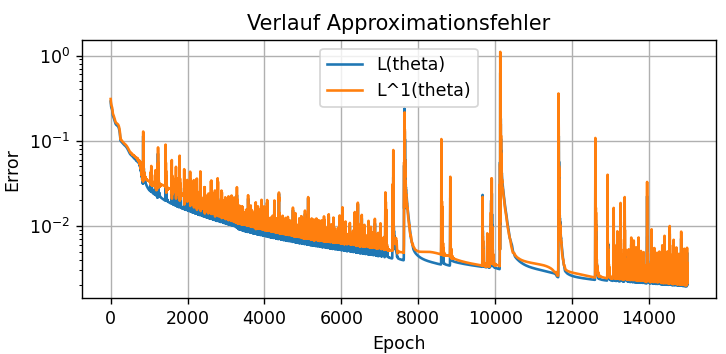
\includegraphics[width=0.7\textwidth]{papers/neuronal/images/approximation_error_burgers.png}
    \caption{Verlauf Approximationsfehler Burgers-Gleichung}
    \label{fig:fehler_burgers}
\end{figure}

Wertet man das neuronale Netzwerk über die Bereiche von $x$ und $t$ aus, ergibt sich ein Plot der Lösung des neuronalen Netzwerks (siehe \ref{fig:loesung_burgers}).

\begin{figure}
    \centering
    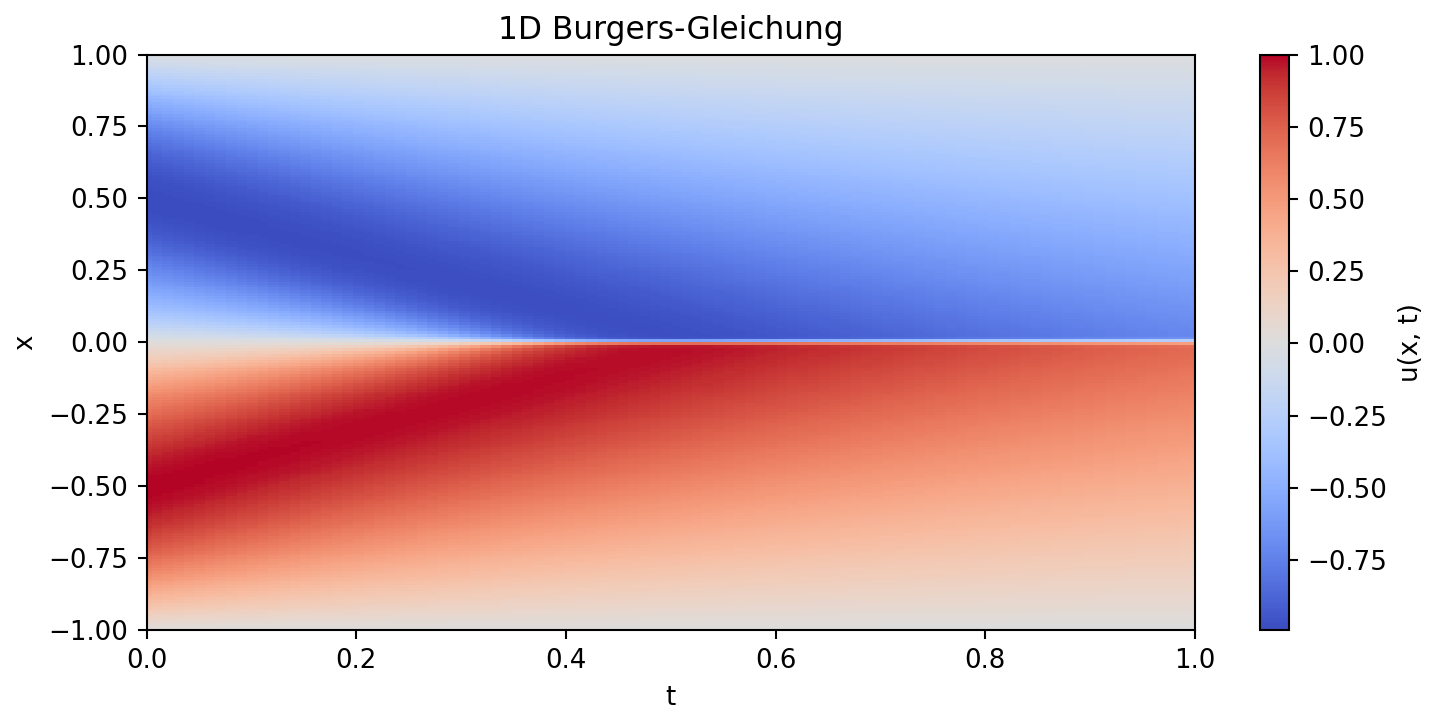
\includegraphics[width=0.8\textwidth]{papers/neuronal/images/prediction_burgers_net.png}
    \caption{Lösungs-Plot Burgers-Gleichung}
    \label{fig:loesung_burgers}
\end{figure}

Der gesamte Code zur Umsetzung ist im Github Repository des Seminars abgelegt \cite{neuronal:github_source_code}.
